\documentclass{beamer}
\usetheme{metropolis}
\usepackage{graphicx}
\usepackage{booktabs}
\usepackage{hyperref}
\usepackage{listings}
\colorlet{shadecolor}{gray!40}

\lstset{
	language=R,
	basicstyle=\ttfamily\small,
	commentstyle=\color{black},
	keywordstyle=\color{blue},
	numbers=left,
	numberstyle=\tiny\color{red},
	stepnumber=1,
	numbersep=5pt,
	backgroundcolor=\color{shadecolor},
	showspaces=false,
	showstringspaces=false,
	showtabs=false,
	frame=single,
	tabsize=2,
	captionpos=b,
	breaklines=true,
	breakatwhitespace=false,
	title=\lstname
}


\newenvironment{bigitemize}{\itemize\addtolength{\itemsep}{10pt}}{\enditemize}
\newcommand\independent{\protect\mathpalette{\protect\independenT}{\perp}}
\def\independenT#1#2{\mathrel{\rlap{$#1#2$}\mkern2mu{#1#2}}}
\title{Microeconometrics Module}
\subtitle{Lecture 3: Endogeneity}
\author{Swapnil Singh}
\date{Lietuvos Bankas and KTU \\ \href{https://github.com/swapnil1987/econometrics-2024}{\textcolor{magenta}{Course Link}}}

\begin{document}
	
	\maketitle
	
\begin{frame}
	\frametitle{Simple Linear Regression}
	\begin{itemize}
		\item Assume that there are two variables -- $y$ and $x$ -- and we are interested in understanding the relationship between them
		\begin{itemize}
			\item $y =$ wage and, $x = $ education
			\item $y =$ diabetes and, $x =$ whether smoking or not
		\end{itemize}
		\item More importantly, we are interested in knowing whether $x$ has a \textbf{causal} effect on $y$
		\item Three things to consider:
		\begin{enumerate}
			\item How to allow other factors to affect $y$?
			\item What is the functional relationship between $y$ and $x$?
			\item Under which conditions we can claim causality?
		\end{enumerate}
	\end{itemize}
\end{frame}


\begin{frame}
	\frametitle{Simple Linear Regression}
	\begin{itemize}
		\item Bite the bullet and write:
		$$ y = \beta_0 + \beta_1 x + u $$
		where $u$ is the error term
		\item Essentially, we are saying that 
		\begin{enumerate}
			\item Other factors affect $y$ additively
			\item Parametric relationship is linear
			\begin{itemize}
				\item Note that even though parametric relationship is linear, it can capture non-linear relationship between $y$ and $x$
			\end{itemize}
		\end{enumerate}
		\item But still there is an open question about causality
		\item For this, we put structure on the relationship between $x$ and $u$
	\end{itemize}
\end{frame}

\begin{frame}
	\frametitle{Simple Linear Regression}
	\begin{itemize}
		\item Two assumptions: (1) $\mathbb E(u) = 0$, and (2) $\mathbb E(u|x) = \mathbb E(u) = 0$
		\item The first assumption is innoccuous
		\item The second assumption is the most important
		\item The violation of second assumption implies endogeneity problem, and we cannot claim causal effect. Why?
	\end{itemize}
	
\end{frame}


\begin{frame}
	\frametitle{Simple Linear Regression}
	\begin{itemize}
		\item Two assumptions: (1) $\mathbb E(u) = 0$, and (2) $\mathbb E(u|x) = \mathbb E(u) = 0$
		\item The first assumption is innoccuous
		\item The second assumption is the most important
		\item The violation of second assumption implies endogeneity problem, and we cannot claim causal effect. Why?
	\end{itemize}
	\begin{figure}
		\centering
		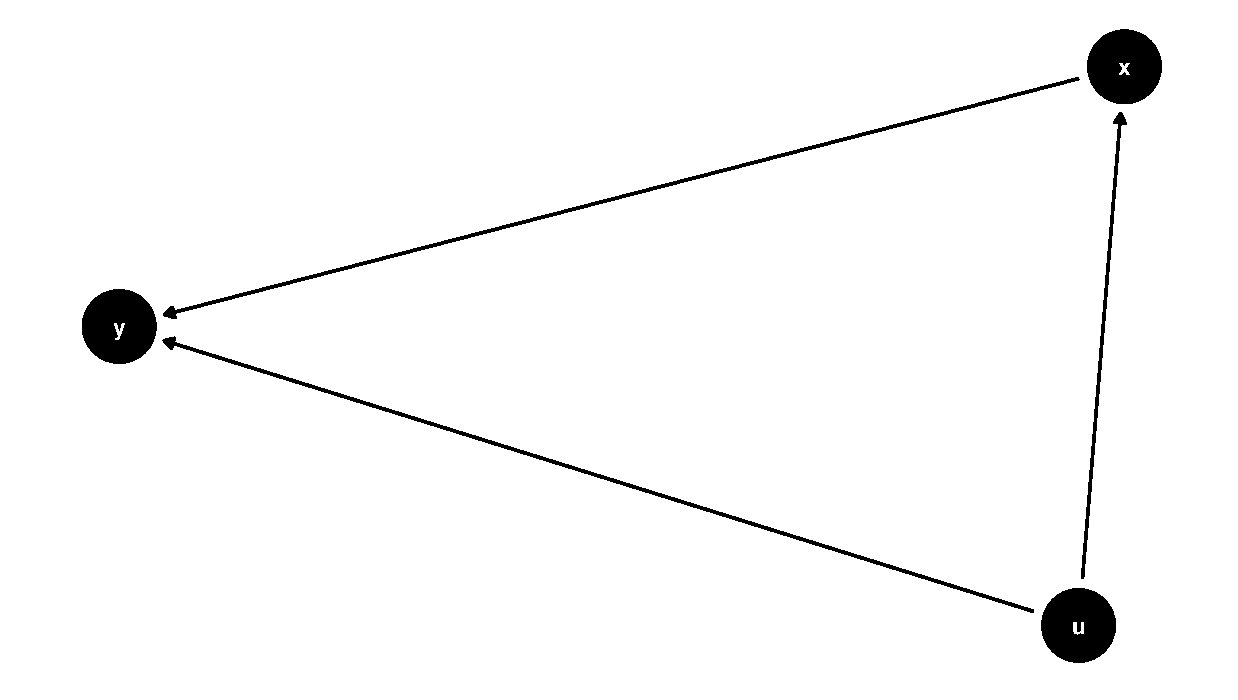
\includegraphics[scale=0.35]{figures/dag_simple_regression.pdf}
	\end{figure}
\end{frame}


\begin{frame}[fragile]
	\frametitle{Example: Omitted Variable Bias}
	\begin{lstlisting}
		#preliminaries (just FYI, as I am displaying code for the first time)
		rm(list=ls())
		gc()
		setwd(dirname(rstudioapi::getActiveDocumentContext()$path))
		Sys.setenv(lang='en')
	\end{lstlisting}
	
\end{frame}


\begin{frame}[fragile]
	\frametitle{Example: Omitted Variable Bias}
	\begin{lstlisting}
		
		# Setting up the data
		set.seed(123)
		N <- 1000
		X1 <- rnorm(N, 50, 10) # Explanatory variable
		U <- rnorm(N, 0, 5)   # Unobserved variable
		X2 <- 0.5 * X1 + rnorm(N,1,6)     # Another explanatory variable
		Y <- 2 + 1 * X1 + 1.5 * X2 + U # Outcome variable
	\end{lstlisting}
\end{frame}


\begin{frame}
		\frametitle{Example: Omitted Variable Bias}
	\small
	\begin{table} \centering 
		\resizebox{\linewidth}{!}{
		\begin{tabular}{lcc} 
\bottomrule\bottomrule 
			Dependent variable:& \multicolumn{2}{c}{Y}  \\ 
			\cmidrule(lr){2-3}
			 & (1) & (2)\\ 
			\hline
			X1 & 1.777$^{***}$ & 1.032$^{***}$ \\ 
			& (0.033) & (0.021) \\ 
			X2 &  & 1.524$^{***}$ \\ 
			&  & (0.027) \\ 
			Constant & 2.184 & $-$0.031 \\ 
			& (1.675) & (0.822) \\ 
			& & \\ 
			Observations & 1,000 & 1,000 \\ 
			R$^{2}$ & 0.747 & 0.939 \\ 
			\textit{Note:}  & \multicolumn{2}{r}{$^{*}$p$<$0.1; $^{**}$p$<$0.05; $^{***}$p$<$0.01} \\  \bottomrule\bottomrule
		\end{tabular} }
	\end{table} 
\end{frame}


\begin{frame}
	\frametitle{Point of Caution}
	\begin{itemize}
		\item Endogeneity is a conceptual issue
			\begin{itemize}
				\item Cannot test it by using \textcolor{red}{residuals} after running the OLS regression
			\end{itemize}
	\end{itemize}
\end{frame}

\begin{frame}
	\frametitle{Point of Caution}
	\begin{figure}
		\centering
		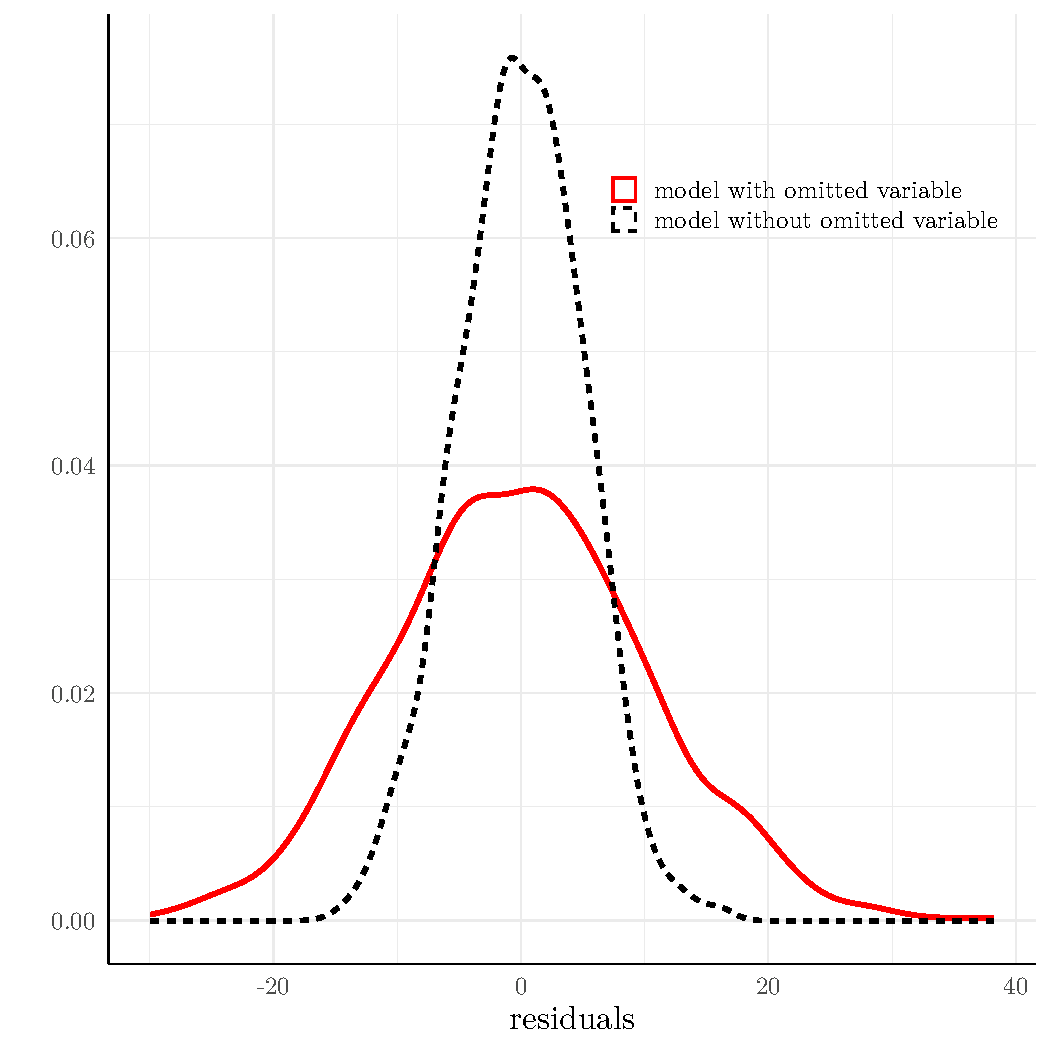
\includegraphics[width=0.7\linewidth]{figures/ovb-residuals}
	\end{figure}
\end{frame}


\begin{frame}
	\frametitle{Point of Caution}
	\begin{itemize}
		\item Endogeneity is a conceptual issue
		\begin{itemize}
			\item Cannot test it by using \textcolor{red}{residuals} after running the OLS regression
		\end{itemize}
		\item You cannot compute \textcolor{red}{error} term, i.e. $u$, but you will always get residuals after running the regression
		\item Remember, source of endogeneity is $\mathbb E(u|x) \neq 0$
	\end{itemize}
\end{frame}








\end{document}